\setcounter{chapter}{0}
\chapter{Sample Chapter}
\label{chap:sample-chapter} % Label for reference.

Here, we use all the additional functionalities available in this template over the \verb|tuftebook| template; some may be redundant. Most of the initial example usages are specific to mathematics as was originally intended by Gilles. In later versions, we will add more example uses for notes specific to CS, programming, machine learning etc. Look at \verb|main.tex| for information on how to use the different features in the template.

% Starting a section

\section*{Sample Section}
% Subsection
\subsection*{Sample Subsection}

Colorful boxes for various theorem-type text. These can be changed to simple boxed ones too, check \verb|preamble.tex|.

\vspace{5mm}

% Sample definition

\textcolor{red}{Use} \verb|\begin{definition} \end{definition}| \textcolor{red}{to write a definition.}

\begin{definition}[Sample Definition]
	This is the content of the definition. Use \verb|\sidenotemark| here.\sidenotemark
\end{definition}

% Adding sidenote text.
\textcolor{red}{Use} \verb|\sidenotetext| \textcolor{red}{to add text to the sidenote.}
\sidenotetext{I am a sidenote.}

% Adding a lemma

\begin{lemma}[Sample Lemma]
	Use me to prove a larger result.
\end{lemma}

% Adding a proof
\textcolor{red}{Use} \verb|\begin{myproof} \end{myproof}| \textcolor{red}{environment for beginning a proof.}


\begin{myproof}
	The proof is trivial and is left as an exercise to the reader.
\end{myproof}

\textcolor{red}{Use} \verb|\begin{theorem} \end{theorem}| \textcolor{red}{to write a theorem.}

% Adding a theorem
\begin{theorem}[An amazing theorem about something]
	It took mathematicians 42 years to prove me.
\end{theorem}

\textcolor{red}{Use} \verb|\begin{prop} \end{prop}| \textcolor{red}{to write a proposition.}

\begin{prop}
	I get a beautifully typeset document, you tell me ways to make it better.
\end{prop}

\textcolor{red}{Use} \verb|\begin{eg} \end{eg}| \textcolor{red}{to write an example.}

\begin{eg}[An Example.]
	This is an example usage of an example environment.
\end{eg}

\subsubsection{Citation}

% Adding a bibliography reference

Here are a few ways to cite a reference.
\begin{itemize}
	\item Using \verb|\fullcite| $-$ \fullcite{milnor}.
	\item Using \verb|\sidecite| $-$ \sidecite[]{milnor}.
	\item Using \verb|\cite| $-$ \cite{milnor}.
\end{itemize}

\section*{Figures}

\begin{figure*}[h]
	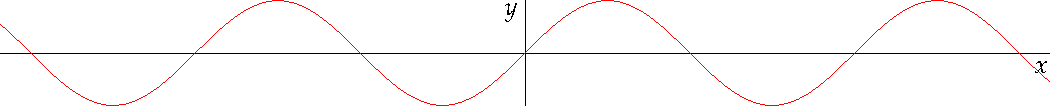
\includegraphics[width=\linewidth]{sine.pdf}%
	\caption{This graph shows $y = \sin x$ from about $x = [-10, 10]$.
		\emph{Notice that this figure takes up the full page width.}}%
	\label{fig:fullfig}%
\end{figure*}

\begin{figure}
	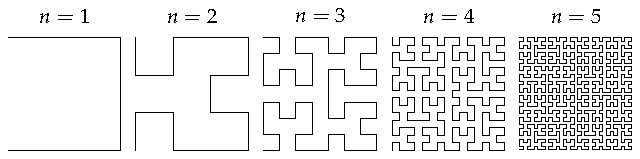
\includegraphics{hilbertcurves.pdf}
	%  \checkparity This is an \pageparity\ page.%
	\caption[Hilbert curves of various degrees $n$.][6pt]{Hilbert curves of various degrees $n$. \emph{Notice that this figure only takes up the main textblock width.}}
	\label{fig:textfig}
	%\zsavepos{pos:textfig}
\end{figure}

